\documentclass{article}

\usepackage{style}
\usepackage{rotating}
\usepackage[labelformat=empty]{caption}
\usepackage{siunitx}
\usepackage{hyperref}
\newcommand{\tb}{\textbullet}
\newcommand{\cb}{$\circ$}
\newcommand{\rgbnote}{Note: Red, green, and blue arrows correspond to $x$, $y$, and $z$ axes, respectfully.}

\lhead{MEEN 612: Project}
\rhead{Bryan Yaggi}

\begin{document}

\section{Mechanical Design}
\begin{itemize}
  \item Design commentary
    \begin{itemize}
      \item 7R spatial
    \end{itemize}
  \item Selfies
\end{itemize}

\begin{figure}[H]
  \centering
  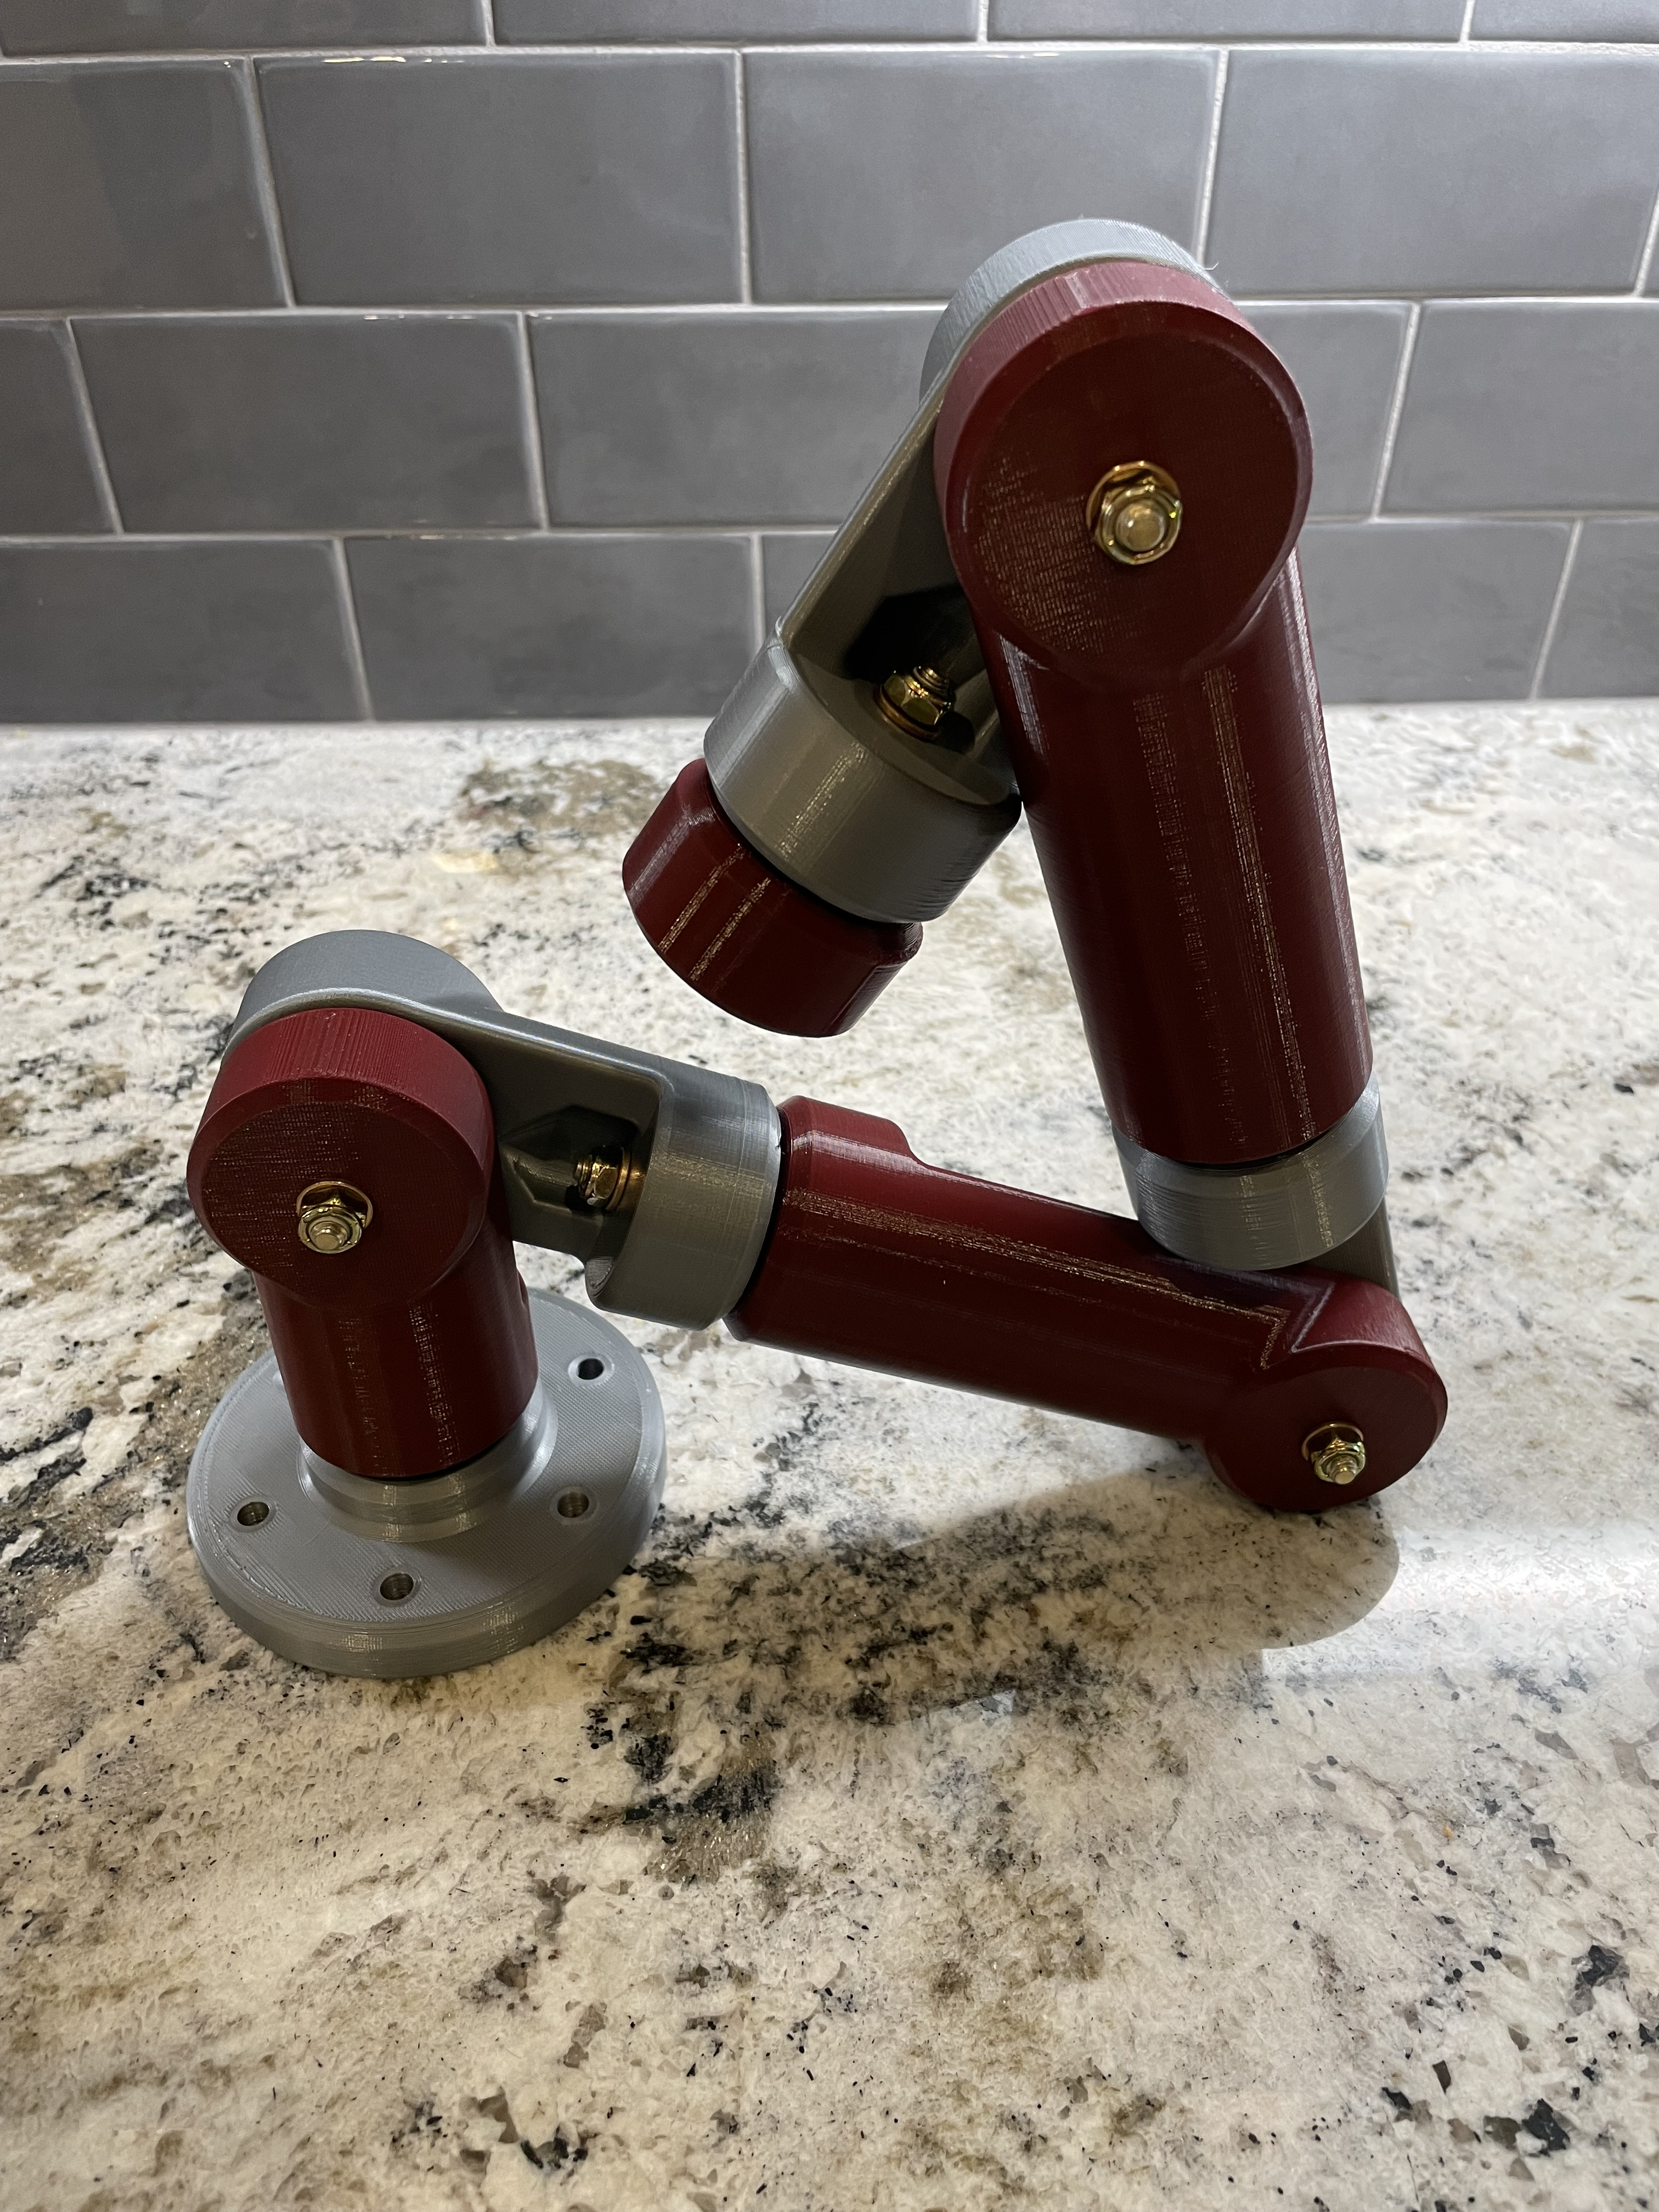
\includegraphics[width=0.25\linewidth]{counter1}
  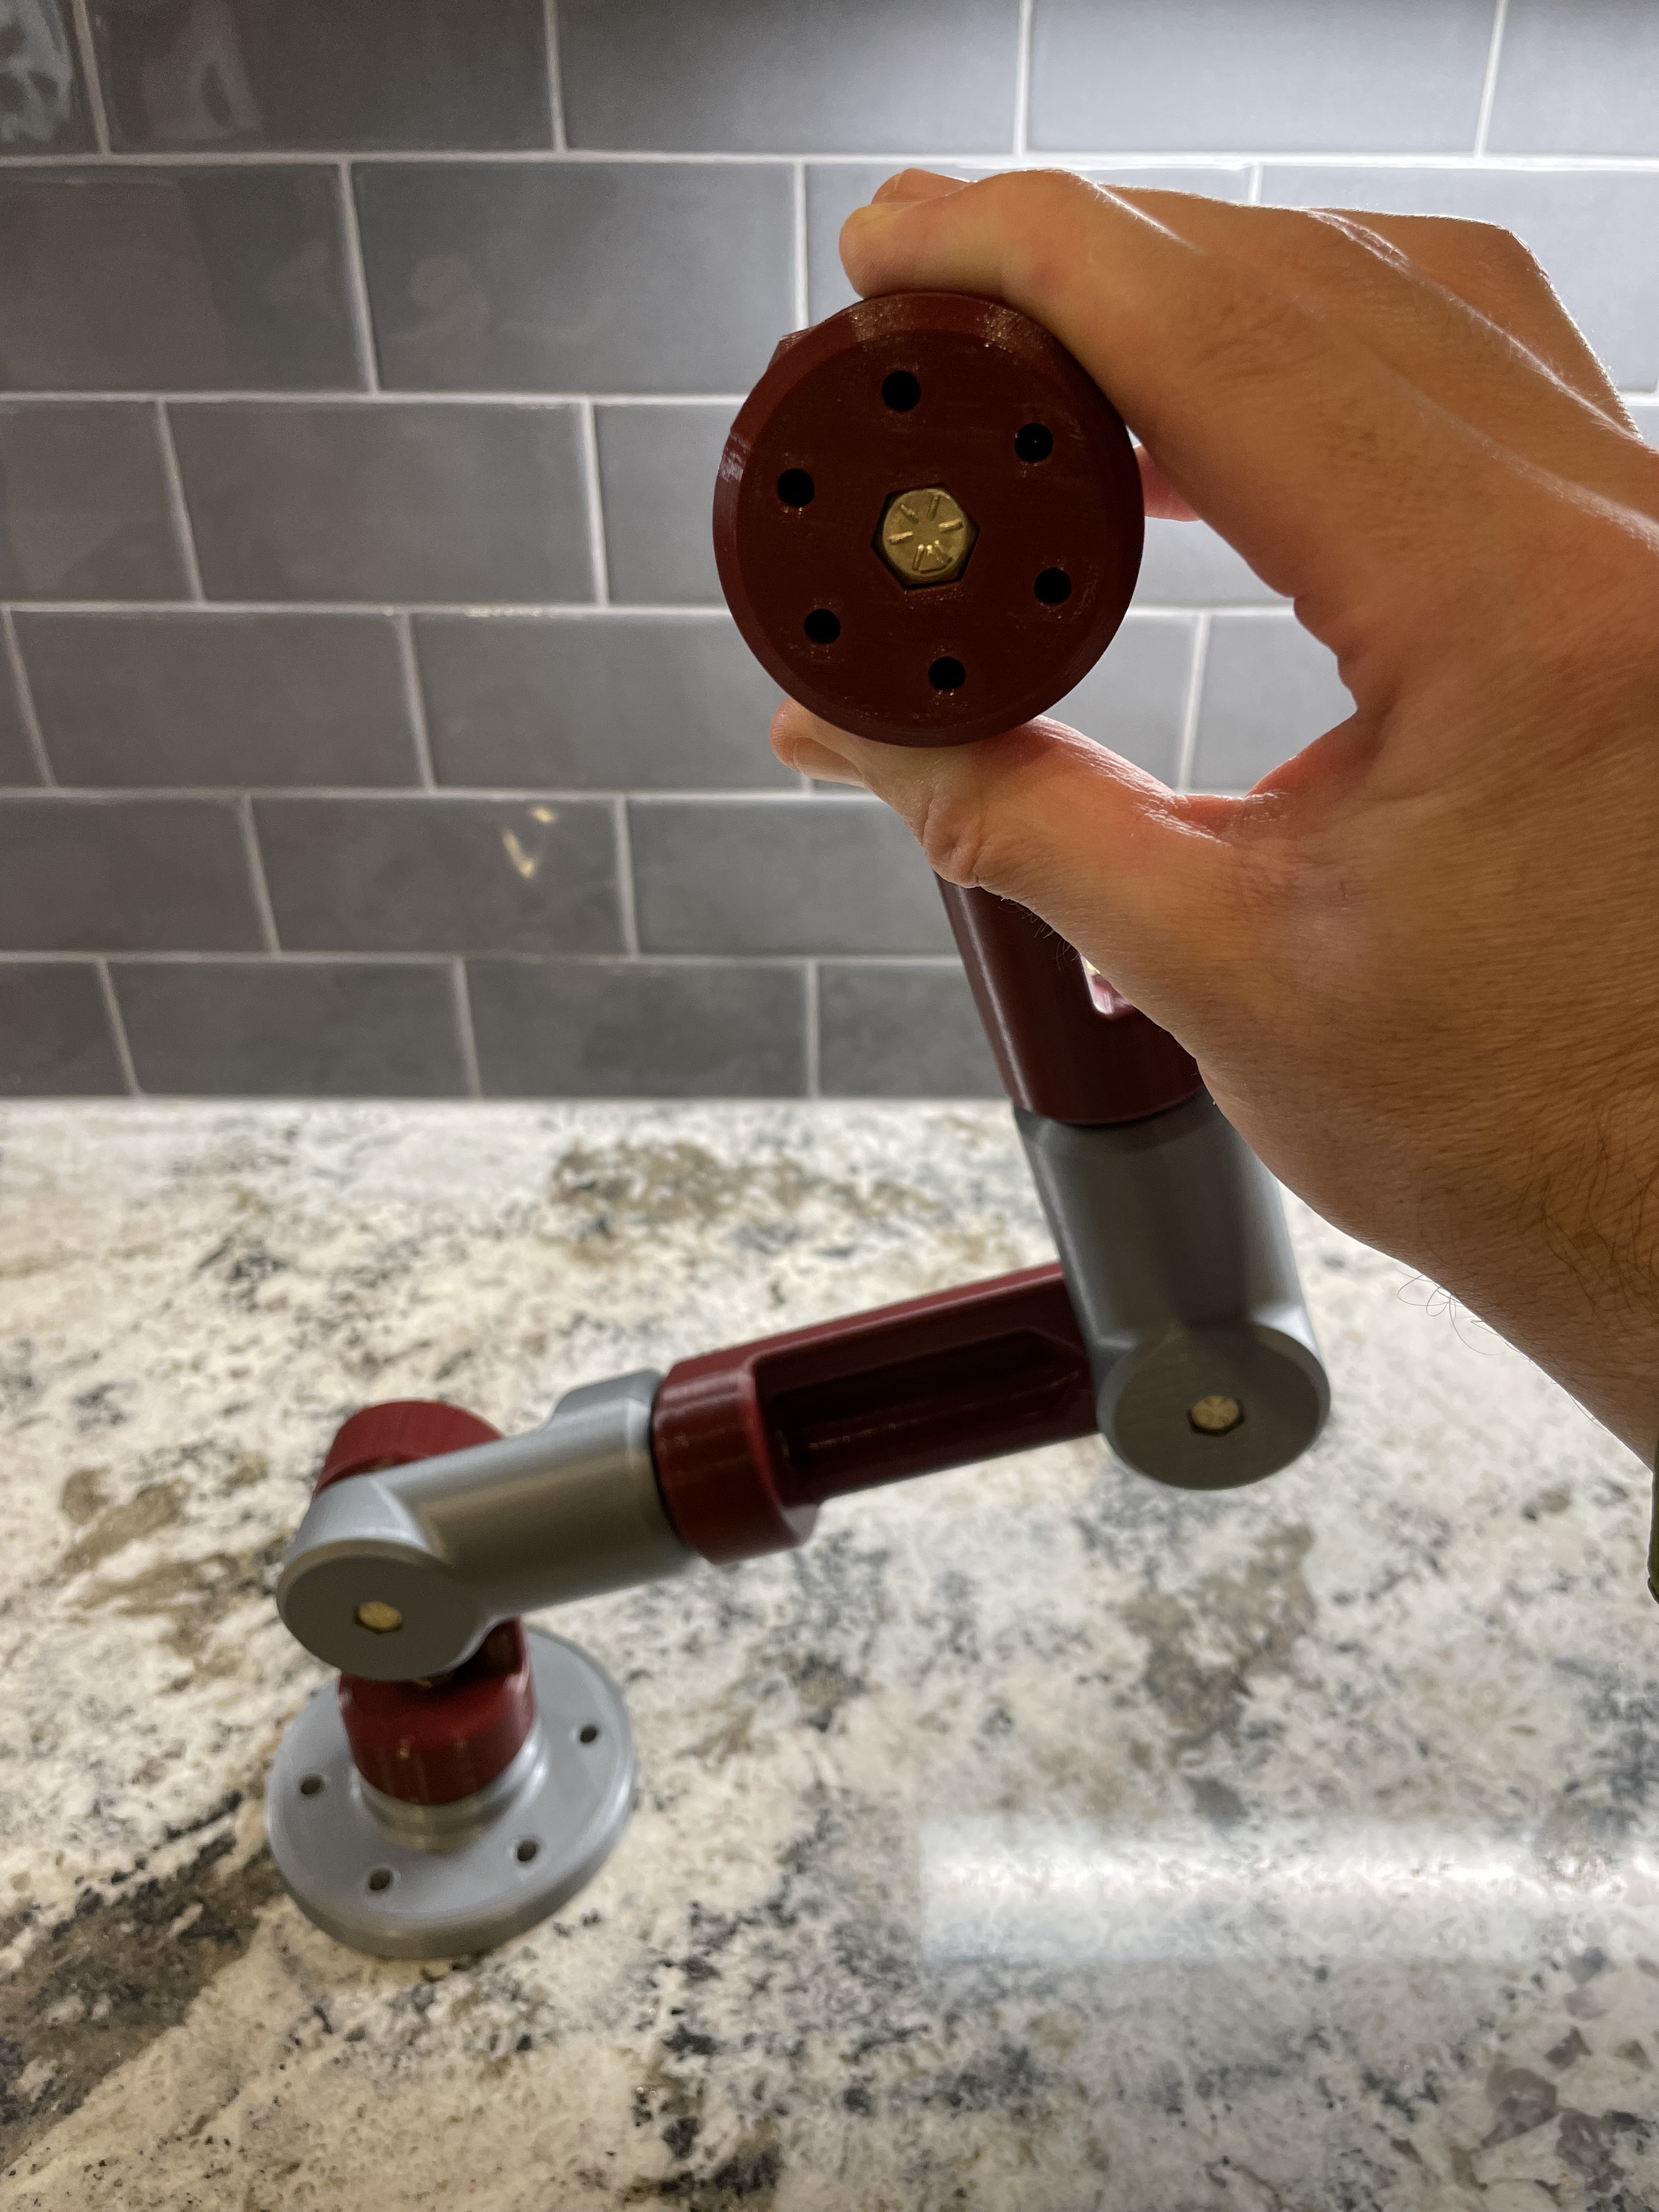
\includegraphics[width=0.25\linewidth]{counter2}
  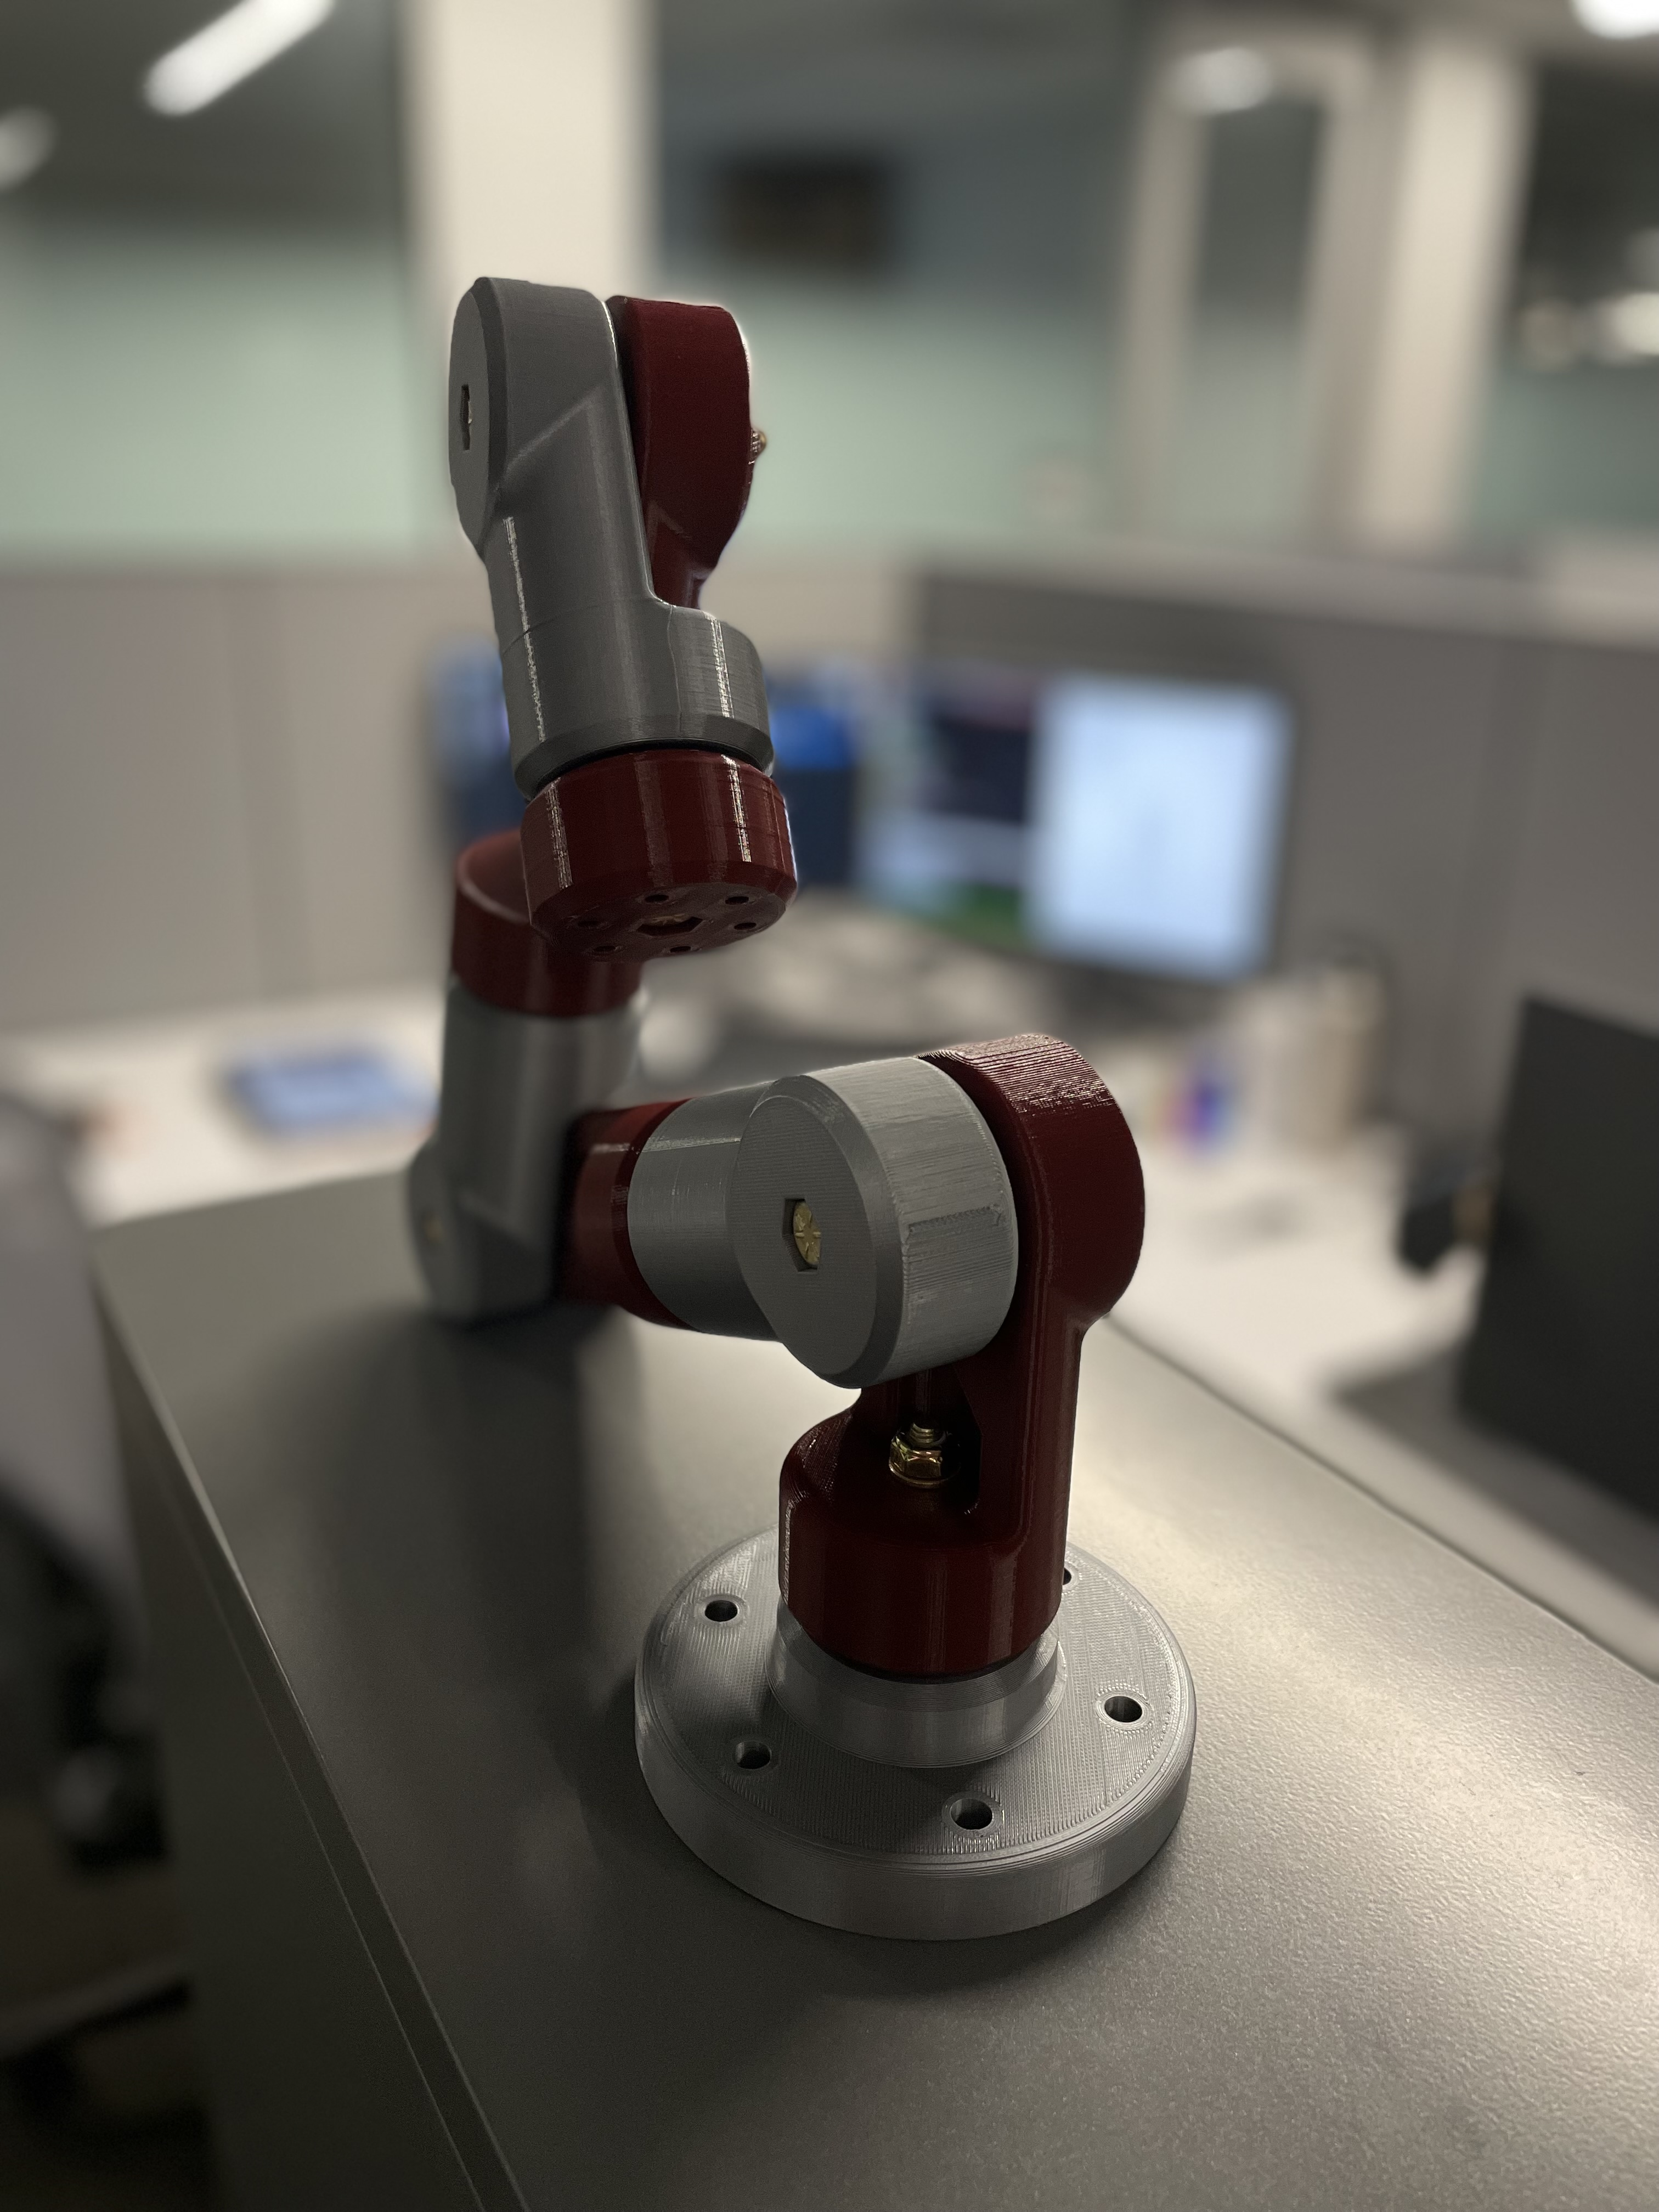
\includegraphics[width=0.25\linewidth]{ric1}
  \caption{Physical manipulator}
\end{figure}

\section{Kinematics}
\begin{itemize}
  \item Frame definitions
  \item D-H parameters
  \item Forward kinematics
\end{itemize}
    
\begin{figure}[H]
  \centering
  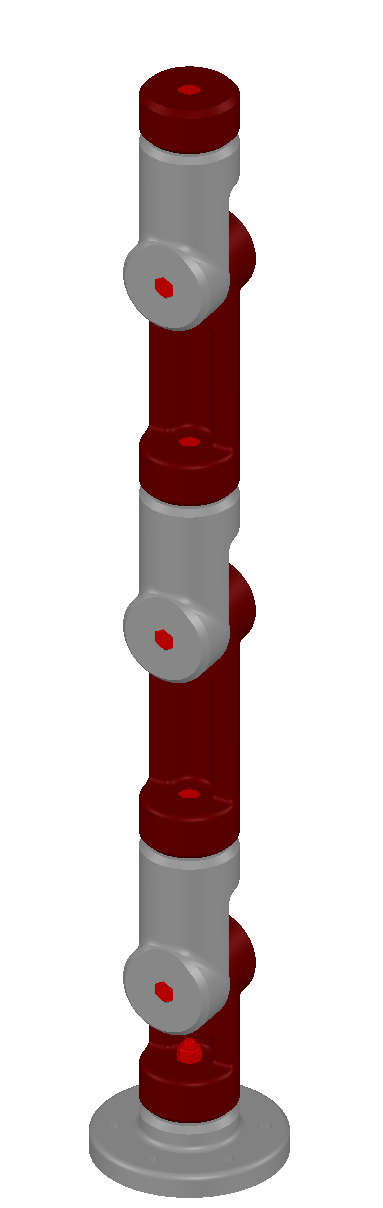
\includegraphics[height=0.5\linewidth]{assembly}
  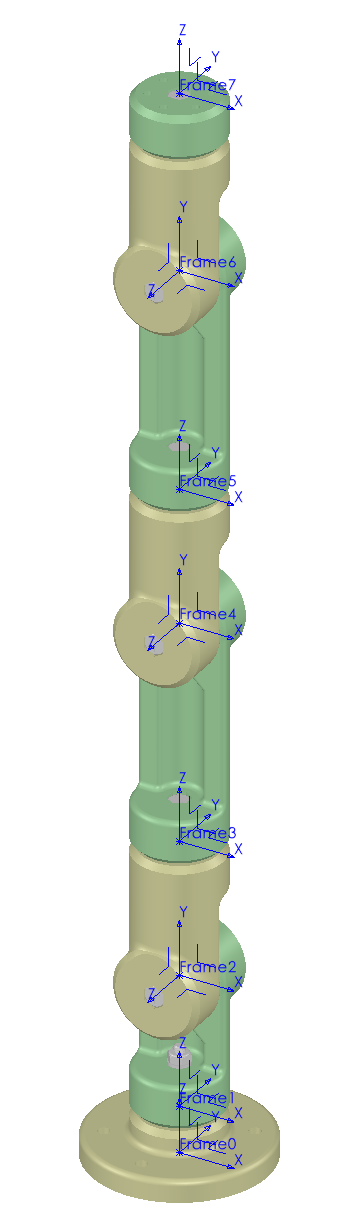
\includegraphics[height=0.5\linewidth]{frames}
  \caption{Frame definitions}
\end{figure}

\begin{center}
\begin{tabular}{|c c c c c|}
  \hline
  Joint $i$ & $\alpha_{i-1}$ & $a_{i-1}$ & $d_i$ & $\theta_i$ \\
  \hline
  1 & $0^\circ$ & 0 & $l_1 + b$ & $q_1$ \\
  2 & $90^\circ$ & $l_2$ & 0 & $q_2$ \\
  3 & $-90^\circ$ & 0 & $l_2 + b$ & $q_3$ \\
  4 & $90^\circ$ & $l_3$ & 0 & $q_4$ \\
  5 & $-90^\circ$ & 0 & $l_2 + b$ & $q_5$ \\
  6 & $90^\circ$ & $l_3$ & 0 & $q_6$ \\
  7 & $-90^\circ$ & 0 & $l_1 + l_2 + b$ & $q_7$ \\
  \hline
\end{tabular}
\end{center}
where $b = \frac{1}{16}"$ is the plain bearing flange thickness, $l_1 = 1"$, $l_2 = 3"$, and $l_3 = 5"$.

\begin{align*}
  \p{0}{1}T &= \begin{bmatrix}
    cq_1 & -sq_1 & 0 & 0 \\
    sq_1 & cq_1 & 0 & 0 \\
    0 & 0 & 1 & l_1 + b \\
    0 & 0 & 0 & 1
  \end{bmatrix} = \begin{bmatrix}
    cq_1 & -sq_1 & 0 & 0 \\
    sq_1 & cq_1 & 0 & 0 \\
    0 & 0 & 1 & 1.0625 \\
    0 & 0 & 0 & 1
  \end{bmatrix} \\
  \p{1}{2}T &= \begin{bmatrix}
    cq_2 & -sq_2 & 0 & l_2 \\
    0 & 0 & -1 & 0 \\
    sq_2 & cq_2 & 0 & 0 \\
    0 & 0 & 0 & 1
  \end{bmatrix} = \begin{bmatrix}
    cq_2 & -sq_2 & 0 & 3 \\
    0 & 0 & -1 & 0 \\
    sq_2 & cq_2 & 0 & 0 \\
    0 & 0 & 0 & 1
  \end{bmatrix} \\
  \p{2}{3}T = \p{4}{5}T &= \begin{bmatrix}
    cq & -sq & 0 & 0 \\
    0 & 0 & 1 & l_2 + b \\
    -sq & -cq & 0 & 0 \\
    0 & 0 & 0 & 1
  \end{bmatrix} = \begin{bmatrix}
    cq & -sq & 0 & 0 \\
    0 & 0 & 1 & 3.0625 \\
    -sq & -cq & 0 & 0 \\
    0 & 0 & 0 & 1
  \end{bmatrix} \\
  \p{3}{4}T = \p{5}{6}T &= \begin{bmatrix}
    cq & -sq & 0 & l_3 \\
    0 & 0 & -1 & 0 \\
    sq & cq & 0 & 0 \\
    0 & 0 & 0 & 1
  \end{bmatrix} = \begin{bmatrix}
    cq & -sq & 0 & 5 \\
    0 & 0 & -1 & 0 \\
    sq & cq & 0 & 0 \\
    0 & 0 & 0 & 1
  \end{bmatrix} \\
  \p{6}{7}T &= \begin{bmatrix}
    cq_7 & -sq_7 & 0 & 0 \\
    0 & 0 & 1 & l_1 + l_2 + b \\
    -sq_7 & -cq_7 & 0 & 0 \\
    0 & 0 & 0 & 1
  \end{bmatrix} = \begin{bmatrix}
    cq_7 & -sq_7 & 0 & 0 \\
    0 & 0 & 1 & 4.0625 \\
    -sq_7 & -cq_7 & 0 & 0 \\
    0 & 0 & 0 & 1
  \end{bmatrix}
\end{align*}
where $q = q_i$ for $\p{i-1}{i}T$.

\section{Control}
\begin{itemize}
  \item Description
  \item Lyapunov stability proof
  \item Impluse respose plots
\end{itemize}

\href{./downflop_bullet.mp4}{downflop\_bullet.mp4}

\href{./upflop_bullet.mp4}{upflop\_bullet.mp4}

\end{document}
